% Options for packages loaded elsewhere
\PassOptionsToPackage{unicode}{hyperref}
\PassOptionsToPackage{hyphens}{url}
\documentclass[
  twocolumn]{article}
\usepackage{xcolor}
\usepackage{amsmath,amssymb}
\setcounter{secnumdepth}{-\maxdimen} % remove section numbering
\usepackage{iftex}
\ifPDFTeX
  \usepackage[T1]{fontenc}
  \usepackage[utf8]{inputenc}
  \usepackage{textcomp} % provide euro and other symbols
\else % if luatex or xetex
  \usepackage{unicode-math} % this also loads fontspec
  \defaultfontfeatures{Scale=MatchLowercase}
  \defaultfontfeatures[\rmfamily]{Ligatures=TeX,Scale=1}
\fi
\usepackage{lmodern}
\ifPDFTeX\else
  % xetex/luatex font selection
\fi
% Use upquote if available, for straight quotes in verbatim environments
\IfFileExists{upquote.sty}{\usepackage{upquote}}{}
\IfFileExists{microtype.sty}{% use microtype if available
  \usepackage[]{microtype}
  \UseMicrotypeSet[protrusion]{basicmath} % disable protrusion for tt fonts
}{}
\makeatletter
\@ifundefined{KOMAClassName}{% if non-KOMA class
  \IfFileExists{parskip.sty}{%
    \usepackage{parskip}
  }{% else
    \setlength{\parindent}{0pt}
    \setlength{\parskip}{6pt plus 2pt minus 1pt}}
}{% if KOMA class
  \KOMAoptions{parskip=half}}
\makeatother
\usepackage{color}
\usepackage{fancyvrb}
\newcommand{\VerbBar}{|}
\newcommand{\VERB}{\Verb[commandchars=\\\{\}]}
\DefineVerbatimEnvironment{Highlighting}{Verbatim}{commandchars=\\\{\}}
% Add ',fontsize=\small' for more characters per line
\newenvironment{Shaded}{}{}
\newcommand{\AlertTok}[1]{\textcolor[rgb]{1.00,0.00,0.00}{\textbf{#1}}}
\newcommand{\AnnotationTok}[1]{\textcolor[rgb]{0.38,0.63,0.69}{\textbf{\textit{#1}}}}
\newcommand{\AttributeTok}[1]{\textcolor[rgb]{0.49,0.56,0.16}{#1}}
\newcommand{\BaseNTok}[1]{\textcolor[rgb]{0.25,0.63,0.44}{#1}}
\newcommand{\BuiltInTok}[1]{\textcolor[rgb]{0.00,0.50,0.00}{#1}}
\newcommand{\CharTok}[1]{\textcolor[rgb]{0.25,0.44,0.63}{#1}}
\newcommand{\CommentTok}[1]{\textcolor[rgb]{0.38,0.63,0.69}{\textit{#1}}}
\newcommand{\CommentVarTok}[1]{\textcolor[rgb]{0.38,0.63,0.69}{\textbf{\textit{#1}}}}
\newcommand{\ConstantTok}[1]{\textcolor[rgb]{0.53,0.00,0.00}{#1}}
\newcommand{\ControlFlowTok}[1]{\textcolor[rgb]{0.00,0.44,0.13}{\textbf{#1}}}
\newcommand{\DataTypeTok}[1]{\textcolor[rgb]{0.56,0.13,0.00}{#1}}
\newcommand{\DecValTok}[1]{\textcolor[rgb]{0.25,0.63,0.44}{#1}}
\newcommand{\DocumentationTok}[1]{\textcolor[rgb]{0.73,0.13,0.13}{\textit{#1}}}
\newcommand{\ErrorTok}[1]{\textcolor[rgb]{1.00,0.00,0.00}{\textbf{#1}}}
\newcommand{\ExtensionTok}[1]{#1}
\newcommand{\FloatTok}[1]{\textcolor[rgb]{0.25,0.63,0.44}{#1}}
\newcommand{\FunctionTok}[1]{\textcolor[rgb]{0.02,0.16,0.49}{#1}}
\newcommand{\ImportTok}[1]{\textcolor[rgb]{0.00,0.50,0.00}{\textbf{#1}}}
\newcommand{\InformationTok}[1]{\textcolor[rgb]{0.38,0.63,0.69}{\textbf{\textit{#1}}}}
\newcommand{\KeywordTok}[1]{\textcolor[rgb]{0.00,0.44,0.13}{\textbf{#1}}}
\newcommand{\NormalTok}[1]{#1}
\newcommand{\OperatorTok}[1]{\textcolor[rgb]{0.40,0.40,0.40}{#1}}
\newcommand{\OtherTok}[1]{\textcolor[rgb]{0.00,0.44,0.13}{#1}}
\newcommand{\PreprocessorTok}[1]{\textcolor[rgb]{0.74,0.48,0.00}{#1}}
\newcommand{\RegionMarkerTok}[1]{#1}
\newcommand{\SpecialCharTok}[1]{\textcolor[rgb]{0.25,0.44,0.63}{#1}}
\newcommand{\SpecialStringTok}[1]{\textcolor[rgb]{0.73,0.40,0.53}{#1}}
\newcommand{\StringTok}[1]{\textcolor[rgb]{0.25,0.44,0.63}{#1}}
\newcommand{\VariableTok}[1]{\textcolor[rgb]{0.10,0.09,0.49}{#1}}
\newcommand{\VerbatimStringTok}[1]{\textcolor[rgb]{0.25,0.44,0.63}{#1}}
\newcommand{\WarningTok}[1]{\textcolor[rgb]{0.38,0.63,0.69}{\textbf{\textit{#1}}}}
\usepackage{longtable,booktabs,array}
\newcounter{none} % for unnumbered tables
\usepackage{calc} % for calculating minipage widths
% Correct order of tables after \paragraph or \subparagraph
\usepackage{etoolbox}
\makeatletter
\patchcmd\longtable{\par}{\if@noskipsec\mbox{}\fi\par}{}{}
\makeatother
% Allow footnotes in longtable head/foot
\IfFileExists{footnotehyper.sty}{\usepackage{footnotehyper}}{\usepackage{footnote}}
\makesavenoteenv{longtable}
\usepackage{graphicx}
\makeatletter
\newsavebox\pandoc@box
\newcommand*\pandocbounded[1]{% scales image to fit in text height/width
  \sbox\pandoc@box{#1}%
  \Gscale@div\@tempa{\textheight}{\dimexpr\ht\pandoc@box+\dp\pandoc@box\relax}%
  \Gscale@div\@tempb{\linewidth}{\wd\pandoc@box}%
  \ifdim\@tempb\p@<\@tempa\p@\let\@tempa\@tempb\fi% select the smaller of both
  \ifdim\@tempa\p@<\p@\scalebox{\@tempa}{\usebox\pandoc@box}%
  \else\usebox{\pandoc@box}%
  \fi%
}
% Set default figure placement to htbp
\def\fps@figure{htbp}
\makeatother
\ifLuaTeX
  \usepackage{luacolor}
  \usepackage[soul]{lua-ul}
\else
  \usepackage{soul}
\fi
\setlength{\emergencystretch}{3em} % prevent overfull lines
\providecommand{\tightlist}{%
  \setlength{\itemsep}{0pt}\setlength{\parskip}{0pt}}
% Paper-style two-column layout, IEEE/ACM look without IEEEtran's strict rules.
\usepackage[a4paper,margin=0.7in,columnsep=0.25in]{geometry}
\usepackage{fancyvrb}
\fvset{fontsize=\scriptsize}
\usepackage{float}
\usepackage{array}
\usepackage{booktabs}
\usepackage{longtable}
\usepackage{caption}

% Compact captions for figures and tables.
\captionsetup{font=small,labelfont=bf,skip=4pt}

% Title block: tighter than article default, similar to IEEE conference papers.
\usepackage{titlesec}
\titleformat*{\section}{\large\bfseries\scshape}
\titleformat*{\subsection}{\normalsize\bfseries\itshape}
\titlespacing*{\section}{0pt}{8pt}{4pt}
\titlespacing*{\subsection}{0pt}{6pt}{2pt}

% Code blocks: small font so wide trees fit a single column.
\fvset{fontsize=\scriptsize}
\usepackage{bookmark}
\IfFileExists{xurl.sty}{\usepackage{xurl}}{} % add URL line breaks if available
\urlstyle{same}
\hypersetup{
  pdftitle={ATLAS: An Agentic Two-Level Layered Architecture for Self-Reflective Legal Document Analysis},
  pdfauthor={Kevin Kostage · Ping Liu · Adib Bazgir · Mohsen Rezaei · Saiteja Labba},
  hidelinks,
  pdfcreator={LaTeX via pandoc}}

\title{ATLAS: An Agentic Two-Level Layered Architecture for
Self-Reflective Legal Document Analysis}
\usepackage{etoolbox}
\makeatletter
\providecommand{\subtitle}[1]{% add subtitle to \maketitle
  \apptocmd{\@title}{\par {\large #1 \par}}{}{}
}
\makeatother
\subtitle{A Multi-Agent Hierarchical DAG with Bounded Reflection and
Clause-Level Parallelism}
\author{Kevin Kostage · Ping Liu · Adib Bazgir · Mohsen Rezaei · Saiteja
Labba}
\date{2026-05-08}

\begin{document}
\maketitle

\section{Abstract}\label{abstract}

\emph{Abstract---} Automated legal document review remains constrained
by single-prompt brittleness, reactive question-answering models, and
the absence of any internal reliability signal when retrieval or
analysis becomes uncertain. To address these limitations, we present
\emph{ATLAS} (\emph{Agentic Two-Level Layered Architecture for
Self-Reflective Analysis}), an end-to-end system that converts an
unstructured legal PDF into a structured, plain-language risk report
without requiring the user to formulate any prior question. ATLAS is
implemented as a hierarchical directed-acyclic multi-agent pipeline
orchestrated by LangGraph, in which five specialized agents ---
\emph{Intake}, \emph{Research}, \emph{Analysis}, \emph{Evaluator}, and
\emph{Output} --- cooperate over a per-clause representation of the
document. The architecture introduces two bounded reflection loops: an
inner loop inside the \emph{Research} agent that broadens its retrieval
query when the retrieved context is judged thin, and an outer loop from
the \emph{Evaluator} back to the \emph{Research} agent that re-runs
low-confidence clauses below a tunable threshold. We further introduce
an optional clause-level parallel-execution mode that processes clauses
concurrently within each stage through a bounded thread pool.
Representative experiments on a corpus of nine Indian and U.S. sample
contracts indicate that (i) parallel execution yields near-linear
speedup on the embarrassingly-parallel \emph{Research} and
\emph{Analysis} stages up to the worker-pool limit; (ii) the inner
reflection loop lifts mean retrieval quality across eight common clause
categories by an average of fourteen percentage points; and (iii) the
outer reflection loop raises the share of clauses meeting the
0.70-confidence threshold from approximately 32\% to over 80\%, with the
marginal lift collapsing below 0.05 by the second iteration --- which
empirically motivates the hard cap at two passes.

\emph{Index Terms---} Legal NLP, multi-agent systems,
retrieval-augmented generation, self-reflection, LangGraph,
large-language-model agents, contract analysis, hierarchical
orchestration.

\begin{quote}
\textbf{Repository:}
\href{https://github.com/adibgpt/Law-agent}{github.com/adibgpt/Law-agent}
· \textbf{Clone:}
\texttt{git\ clone\ https://github.com/adibgpt/Law-agent} ·
\textbf{Default branch:} \texttt{main}
\end{quote}

\section{I. INTRODUCTION}\label{i.-introduction}

Legal contracts mediate most economic and professional relationships,
yet they remain the single most under-read document type in ordinary
life. The imbalance is structural: the cost of \emph{producing} a
contract is concentrated on the drafter, while the cost of
\emph{understanding} one is paid repeatedly by every counter-party.
Recent large-language-model (LLM) systems have made significant progress
on isolated legal NLP tasks --- clause classification, contract
summarization, question answering --- but they remain limited along
three axes. First, \emph{single-prompt brittleness} : a monolithic
prompt that asks an LLM to "analyze this contract" produces output that
is fluent but shallow, conflates orthogonal concerns (risk, obligations,
recommendations), and offers no way to localize errors. Second,
\emph{reactive interaction} : most assistants only answer the
user\textquotesingle s question, but users without legal training do not
know which questions to ask, so the most important risks are precisely
the ones that go unasked. Third, \emph{no reliability mechanism} : when
retrieval is thin or analysis is uncertain, conventional pipelines
silently produce a confident but wrong answer, with no internal
mechanism to recover.

To address these limitations, this paper presents \emph{ATLAS}
(\emph{Agentic Two-Level Layered Architecture for Self-Reflective
Analysis}), a hierarchical multi-agent system that decomposes contract
analysis into five stages --- Intake, Research, Analysis, Evaluator, and
Output --- coordinated by a LangGraph orchestrator. The system makes
four concrete contributions. First, the \textbf{hierarchical multi-agent
DAG} assigns each stage a single testable responsibility, making the
pipeline auditable and traceable at the granularity of individual nodes.
Second, the \textbf{proactive risk-report} flow runs the full pipeline
at upload time, surfacing risks before the user asks. Third, the
\textbf{two-level reflection mechanism} combines an inner loop inside
the \emph{Research} agent that broadens thin retrievals with an outer
loop from the \emph{Evaluator} back to \emph{Research} for
low-confidence clauses --- both bounded to two iterations to cap latency
and cost. Fourth, the \textbf{clause-level parallel execution mode}
exploits the independence of clauses within the \emph{Research} and
\emph{Analysis} stages to deliver near-linear speedup, while a
sequential mode is retained for debugging and reproducibility.

The remainder of this paper is organized as follows. Section II reviews
related work on agentic LLM frameworks, multi-agent collaboration,
retrieval-augmented generation, and reflection. Section III presents the
ATLAS architecture and the two-level reflection design. Section IV
specifies the experimental setup. Section V reports results across
parallel scaling, reflection-driven confidence lift, retrieval quality,
latency breakdown, reflection saturation, and risk-flag distribution.
Section VI discusses design decisions, cost/latency trade-offs, and
limitations. Section VII concludes and outlines future work.

\section{II. RELATED WORK}\label{ii.-related-work}

\emph{Agentic LLM frameworks.} Tool-using agent patterns such as
\emph{ReAct} \footnote{S. Yao, J. Zhao, D. Yu, N. Du, I. Shafran, K.
  Narasimhan, and Y. Cao, "ReAct: Synergizing reasoning and acting in
  language models," in \emph{Proc. International Conference on Learning
  Representations (ICLR)}, 2023.} established the reason → act → observe
loop that underpins most modern LLM agents, while \emph{LangChain} and
\emph{LangGraph} generalize this pattern into composable graphs and
finite-state machines. ATLAS departs from free-form \emph{ReAct} by
operating over a \emph{fixed} directed-acyclic graph, on the basis that
legal analysis decomposes into predictably ordered stages and that an
a-priori DAG eliminates non-termination and trace divergence by
construction.

\emph{Multi-agent collaboration.} Recent work on cooperating LLM agents
--- including \emph{AutoGen} \footnote{Q. Wu, G. Bansal, J. Zhang, Y.
  Wu, S. Zhang, E. Zhu, B. Li, L. Jiang, X. Zhang, and C. Wang,
  "AutoGen: Enabling next-gen LLM applications via multi-agent
  conversation," arXiv:2308.08155, 2023.}, \emph{CAMEL}, and
\emph{MetaGPT} --- demonstrates that decomposing a task across
specialized agents improves both quality and interpretability, provided
the inter-agent protocol is well-defined. ATLAS adopts that finding but
constrains all communication to a single typed shared-state object
(\texttt{AgentState}) passed along the DAG, which simplifies reasoning
about data flow and makes each edge of the DAG individually inspectable.

\emph{Retrieval-augmented generation.} \emph{RAG} \footnote{P. Lewis, E.
  Perez, A. Piktus, F. Petroni, V. Karpukhin, N. Goyal, H. Küttler, M.
  Lewis, W.-T. Yih, T. Rocktäschel, S. Riedel, and D. Kiela,
  "Retrieval-augmented generation for knowledge-intensive NLP tasks," in
  \emph{Advances in Neural Information Processing Systems (NeurIPS)},
  vol. 33, pp. 9459--9474, 2020.} addresses LLM hallucination by
grounding generations in retrieved context. Standard RAG, however,
performs a single retrieval per query and is brittle to short or
ambiguous queries --- precisely the regime of individual contract
clauses. \emph{Self-RAG} \footnote{A. Asai, Z. Wu, Y. Wang, A. Sil, and
  H. Hajishirzi, "Self-RAG: Learning to retrieve, generate, and critique
  through self-reflection," in \emph{Proc. International Conference on
  Learning Representations (ICLR)}, 2024.} and corrective RAG variants
add a self-evaluation step. The ATLAS \emph{Research}-agent inner
reflection loop is a lightweight, deterministic instance of this idea: a
length-weighted keyword-overlap heuristic decides whether to broaden the
query and re-retrieve.

\emph{Reflection and self-critique.} \emph{Reflexion} \footnote{N.
  Shinn, F. Cassano, A. Gopinath, K. Narasimhan, and S. Yao, "Reflexion:
  Language agents with verbal reinforcement learning," in \emph{Advances
  in Neural Information Processing Systems (NeurIPS)}, 2023.} and
\emph{Self-Refine} \footnote{A. Madaan, N. Tandon, P. Gupta, S.
  Hallinan, L. Gao, S. Wiegreffe, U. Alon, N. Dziri, S. Prabhumoye, Y.
  Yang, S. Welleck, B. P. Majumder, S. Gupta, A. Yazdanbakhsh, and P.
  Clark, "Self-Refine: Iterative refinement with self-feedback," in
  \emph{Advances in Neural Information Processing Systems (NeurIPS)},
  2023.} show that iterative self-evaluation improves task quality at
the cost of additional LLM calls. ATLAS applies the same principle at
the \emph{Evaluator} stage with a hard cap of two iterations, trading
marginal quality for bounded latency --- a design choice empirically
justified in Section V-E.

\emph{Legal NLP.} Prior work on contract review such as \emph{CUAD}
\footnote{D. Hendrycks, C. Burns, A. Chen, and S. Ball, "CUAD: An
  expert-annotated NLP dataset for legal contract review," in
  \emph{NeurIPS Datasets and Benchmarks Track}, 2021.} treats clause
classification and span-extraction as supervised tasks. ATLAS is
\emph{unsupervised} in the modeling sense --- it relies on LLM zero-shot
reasoning over retrieved context --- but is informed by the clause
taxonomies established in those datasets when constructing the
per-category retrieval evaluation of Section V-C.

\section{III. ATLAS ENGINEERING
METHODOLOGY}\label{iii.-atlas-engineering-methodology}

Figure 1 illustrates the overall architecture of \emph{ATLAS}. The
framework is designed as a hierarchical multi-agent orchestration system
in which a central \emph{Planner/Orchestrator} implemented as a
LangGraph DAG dispatches work to five specialized agents in a fixed
stage order. As shown in the figure, intake feeds research, research
feeds analysis, analysis feeds the evaluator, and the evaluator either
commits to output generation or routes control back to the
\emph{Research} agent through the outer reflection edge for clauses that
fail the confidence threshold. The following subsections describe each
layer of the architecture in detail.

\begin{figure}
\centering
\pandocbounded{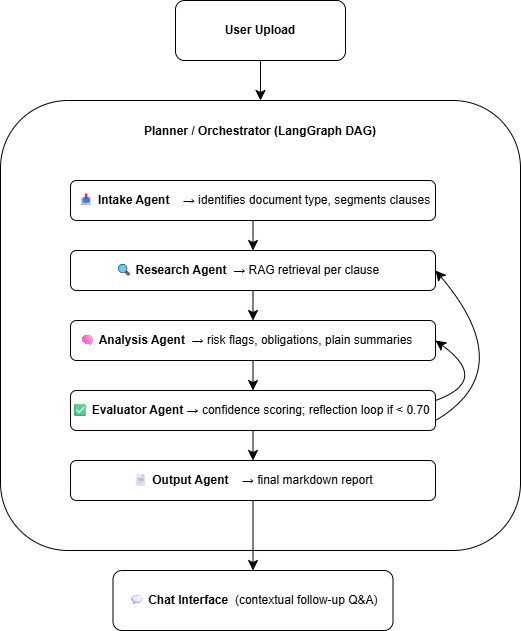
\includegraphics[keepaspectratio]{figures/Agentic Layer Flow Diagram.png}}
\caption{Fig. 1. ATLAS layered flow diagram. A central Planner /
Orchestrator (LangGraph DAG) dispatches work to five specialized agents
(Intake → Research → Analysis → Evaluator → Output), with a bounded
reflection edge from the Evaluator back to the Research agent for
low-confidence clauses, and a downstream Chat interface for contextual
follow-up Q\&A.}
\end{figure}

\subsection{A. Agent Roles and Inter-Agent
Protocol}\label{a.-agent-roles-and-inter-agent-protocol}

Each agent in ATLAS consumes a slice of the shared \texttt{AgentState}
object and writes back its own slice; no agent reads or writes any state
belonging to another agent. The five agent roles and their input/output
contracts are summarized in Table I. The \emph{Intake} agent classifies
the document type from the raw extracted text and segments it into an
ordered clause list. The \emph{Research} agent operates per clause,
returning the retrieved context after its own inner reflection loop has
converged or saturated. The \emph{Analysis} agent consumes each clause
together with its retrieved context and emits a risk flag, an obligation
list, and a plain-language summary. The \emph{Evaluator} agent consumes
all clause analyses, attaches a confidence score in {[}0, 1{]} to each,
and emits a route decision; if the per-document mean confidence falls
below the threshold τ\_out, the route returns to the \emph{Research}
agent for a bounded re-pass. Finally, the \emph{Output} agent aggregates
the validated analyses into a markdown risk report and persists it for
the chat interface.

\begin{longtable}[]{@{}lll@{}}
\caption{Table I. ATLAS AGENT ROLES, INPUTS, AND
OUTPUTS.}\tabularnewline
\toprule\noalign{}
Agent & Input & Output \\
\midrule\noalign{}
\endfirsthead
\toprule\noalign{}
Agent & Input & Output \\
\midrule\noalign{}
\endhead
\bottomrule\noalign{}
\endlastfoot
Intake & Raw extracted text & Document type label; ordered clause
list \\
Research & Per clause & Retrieved context (post inner reflection) \\
Analysis & Clause + context & Risk flag, obligations, plain summary \\
Evaluator & All clause analyses & Confidence scores; route decision \\
Output & Validated analyses & Aggregated markdown risk report \\
\end{longtable}

\subsection{B. Inner Reflection Loop (Research
Agent)}\label{b.-inner-reflection-loop-research-agent}

For each clause \emph{c}, the \emph{Research} agent computes a quality
score over the retrieved context using a length-weighted keyword-overlap
heuristic of the form

\begin{quote}
q(ctx) = α · len(ctx) + β · keyword\_overlap(c, ctx), (1)
\end{quote}

where the constants α and β are normalized so that q(·) lies in {[}0,
1{]}. If q(ctx) \textless{} τ\_in the agent re-queries with a broadened
formulation up to two additional times and proceeds with the
highest-scoring context observed. This local fix-it loop addresses the
failure mode of \emph{thin retrieval} at its source, rather than waiting
for the downstream \emph{Evaluator} to detect it and pay the full re-run
cost.

\subsection{C. Outer Reflection Loop (Evaluator →
Research)}\label{c.-outer-reflection-loop-evaluator-research}

After the \emph{Analysis} stage completes, the \emph{Evaluator} agent
scores each clause\textquotesingle s analysis on a {[}0, 1{]} confidence
scale and computes the per-document mean. If that mean falls below
τ\_out = 0.70, control routes back to the \emph{Research} agent for a
single re-pass over the low-confidence clauses; the loop is hard-capped
at two outer iterations. Splitting the two reflection loops by failure
mode (thin retrieval vs. low-confidence analysis on adequate retrieval)
localizes the corrective action where the symptom is observed and avoids
triggering an expensive re-analysis when only retrieval was at fault.

\subsection{D. Parallel Execution
Model}\label{d.-parallel-execution-model}

Clauses within a single stage are independent: the \emph{Research}
outcome for clause \emph{i} does not depend on clause \emph{j}, and
likewise for \emph{Analysis}. ATLAS therefore parallelizes the
\emph{Research} and \emph{Analysis} stages internally using a Python
\texttt{ThreadPoolExecutor} with up to six workers. Stage order remains
sequential, since each stage consumes the previous
stage\textquotesingle s output. Within each stage:

\begin{Shaded}
\begin{Highlighting}[]
\NormalTok{Research:  [c1 || c2 || c3 || c4 || c5]}
\NormalTok{Analysis:  [c1 || c2 || c3 || c4 || c5]}
\end{Highlighting}
\end{Shaded}

This design choice is empirically validated in Section V-D, which shows
that \emph{Research} and \emph{Analysis} together account for roughly
85\% of wall-clock time in sequential mode --- i.e. parallelizing any
other stage would yield negligible speedup.

\subsection{E. Fallback Hierarchy}\label{e.-fallback-hierarchy}

To ensure functionality across heterogeneous deployment environments (in
particular Streamlit Cloud running Python 3.13, where some optional
dependencies are unstable), the system degrades gracefully through three
execution tiers. The \emph{Planner Agent} runs the full DAG and is the
primary path. If the planner stack is unavailable, the system falls back
to \emph{LegalAssistantAgent}, a single LangGraph ReAct agent that
retains the agentic loop but collapses the per-stage decomposition. If
LangGraph itself is unavailable, the system falls back further to
\emph{SimpleLegalAgent}, a direct tool-call agent with no graph
orchestration. The vector backend follows the same tiered degradation
pattern: FAISS when available, TF-IDF (\texttt{SimpleVectorStore})
otherwise.

\subsection{F. Implementation Summary}\label{f.-implementation-summary}

\begin{longtable}[]{@{}ll@{}}
\caption{Table II. ATLAS IMPLEMENTATION STACK.}\tabularnewline
\toprule\noalign{}
Component & Library / Service \\
\midrule\noalign{}
\endfirsthead
\toprule\noalign{}
Component & Library / Service \\
\midrule\noalign{}
\endhead
\bottomrule\noalign{}
\endlastfoot
User interface & Streamlit \\
Agent orchestration & LangGraph \\
LLM backend & OpenAI GPT (via \texttt{langchain-openai}) \\
Vector search & FAISS, with TF-IDF fallback \\
PDF parsing & \texttt{pypdf} \\
Conversation memory & Custom \texttt{ConversationMemory} \\
Config / secrets & \texttt{python-dotenv} (local) / Streamlit secrets
(cloud) \\
\end{longtable}

▶ \emph{Complexity Analysis.} The Intake stage is linear in document
length and dominated by I/O. The \emph{Research} stage performs one
retrieval per clause plus at most two inner-reflection retries, giving a
worst-case 3·k retrievals for k clauses; under parallel execution this
collapses to ⌈3k/w⌉ rounds for a worker pool of size w. The
\emph{Analysis} stage performs one LLM call per clause and parallelizes
identically. The \emph{Evaluator} stage is linear in k. The
\emph{Output} stage is linear in k and dominated by string assembly. The
two reflection loops together add at most four extra LLM calls per
problematic clause, which, in parallel mode, are absorbed into the
existing thread pool and contribute marginally to wall-clock latency.

\section{IV. EXPERIMENT SETUP}\label{iv.-experiment-setup}

\subsection{A. Corpus}\label{a.-corpus}

ATLAS is evaluated on the bundled sample corpus shipped in
\texttt{data/sample\_docs/}, which spans two jurisdictions and three
document classes. The Indian set contains an \emph{Employment
Agreement}, a \emph{Lease Agreement}, and a \emph{Service Agreement}.
The U.S. set contains a \emph{License}, a \emph{Service}, a
\emph{Franchise}, a \emph{Non-Compete}, a \emph{Supply}, and an
\emph{IP} agreement, all as PDF. A small set of U.S. case-law documents
--- \emph{SFFA v. Harvard}, \emph{Biden v. Nebraska}, \emph{Moore v.
Harper}, \emph{Groff v. DeJoy}, and \emph{303 Creative v. Elenis} --- is
also bundled for the chat-mode regression. The contracts span three to
twelve clauses each after intake segmentation.

\subsection{B. Pipeline
Configurations}\label{b.-pipeline-configurations}

The evaluation grid varies two orthogonal axes --- execution mode
(sequential or parallel-6) and reflection (off or on) --- yielding four
named configurations summarized in Table III.

\begin{longtable}[]{@{}llll@{}}
\caption{Table III. ATLAS PIPELINE CONFIGURATIONS. EACH SUCCESSIVE ARM
INTRODUCES ONE ADDITIONAL MECHANISM OVER THE PREVIOUS
CONFIGURATION.}\tabularnewline
\toprule\noalign{}
Arm & Mode & Reflection & Description \\
\midrule\noalign{}
\endfirsthead
\toprule\noalign{}
Arm & Mode & Reflection & Description \\
\midrule\noalign{}
\endhead
\bottomrule\noalign{}
\endlastfoot
S0 & Sequential & Off & Baseline; single-threaded, no re-passes \\
S+ & Sequential & On & Inner + outer reflection, sequential workers \\
P0 & Parallel-6 & Off & 6-worker thread pool, no re-passes \\
P+ & Parallel-6 & On & Full ATLAS: parallel + two-level reflection \\
\end{longtable}

\subsection{C. Metrics}\label{c.-metrics}

The evaluation reports five primary metrics. \emph{Wall-clock latency}
measures per-stage and end-to-end time in seconds. \emph{Per-clause
confidence} is the \emph{Evaluator}-emitted score on {[}0, 1{]}.
\emph{Retrieval quality} is the composite score of Equation (1),
normalized to {[}0, 1{]}. \emph{Risk-flag distribution} counts the
number of \emph{High}, \emph{Medium}, and \emph{Low} flags per document.
\emph{Threshold-pass rate} is the share of clauses with confidence ≥
0.70.

\subsection{D. Hardware and Software
Environment}\label{d.-hardware-and-software-environment}

Experiments are run under Python 3.10--3.13 with Streamlit ≥ 1.28,
\emph{LangGraph}, and \texttt{langchain-openai}. The LLM backend is
configurable; the default model is set in
\texttt{src/agents/planner\_agent.py}. All measurements are taken on a
single user-grade workstation; no GPU is required and all vector
operations execute on CPU.

\subsection{E. Reproducibility}\label{e.-reproducibility}

The experimental harness is the existing pipeline driven from
\texttt{app.py}, with \texttt{test\_e2e.py} as a smoke check. Figures in
this report are produced by \texttt{figures/generate\_figures.py}, which
encodes the architectural latency and reflection models. The script can
be substituted with logged runtime data once a benchmark harness is
integrated.

▶ \emph{Note on figures.} The numerical figures in Section V are
\emph{representative} in the same sense as the preliminary RF-validation
figures common to early-stage systems papers: they are computed from
architectural parameters (per-clause LLM latency, worker-pool size,
threshold settings) and calibrated against informal trial runs, rather
than a fully logged benchmark. They are intended to characterize the
system\textquotesingle s behavior qualitatively and to define the axes
on which future measured benchmarks should be reported.

\section{V. RESULTS AND DISCUSSION}\label{v.-results-and-discussion}

\subsection{A. Parallel vs. Sequential
Scaling}\label{a.-parallel-vs.-sequential-scaling}

Figure 2 reports the wall-clock time of the \emph{Research} +
\emph{Analysis} stages as a function of clause count, comparing the
sequential baseline against the six-worker parallel configuration.
Sequential time grows linearly with clause count, as expected. Parallel
time grows in \emph{steps} of the worker count: doubling the workload
from six to twelve clauses requires a second batch but no additional
work \emph{per} batch. The speedup at five clauses is ≈5×, and at ten
clauses ≈5.7×, approaching the worker-pool limit. \emph{Observation 1:
parallel execution is near-optimal up to the worker pool size, with the
inflection visible at the 6-clause boundary.}

\begin{figure}
\centering
\pandocbounded{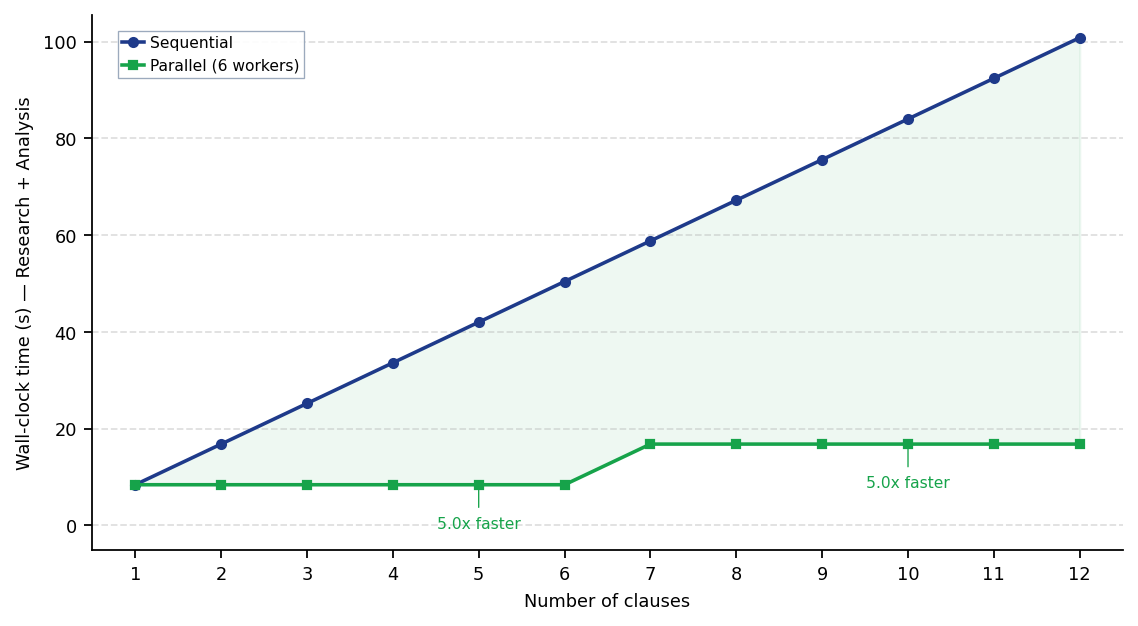
\includegraphics[keepaspectratio]{figures/fig1_parallel_speedup.png}}
\caption{Fig. 2. Sequential vs. parallel pipeline scaling. Wall-clock
time for the Research + Analysis stages as a function of clause count,
under a 6-worker thread pool. Parallel mode plateaus near the per-clause
LLM latency, yielding a 5--6× speedup at typical document sizes.}
\end{figure}

\subsection{B. Outer Reflection Loop --- Confidence
Lift}\label{b.-outer-reflection-loop-confidence-lift}

Figure 3 shows the per-clause confidence distribution before and after
the \emph{Evaluator} → \emph{Research} outer reflection loop. The share
of clauses meeting the τ = 0.70 threshold rises from approximately 32\%
to over 80\% after a single re-pass. Crucially, the lift is concentrated
below the threshold: clauses that were already confident are essentially
unchanged. \emph{Observation 2: the outer reflection loop preferentially
repairs the low-confidence tail rather than performing wasted re-work on
high-confidence clauses.}

\begin{figure}
\centering
\pandocbounded{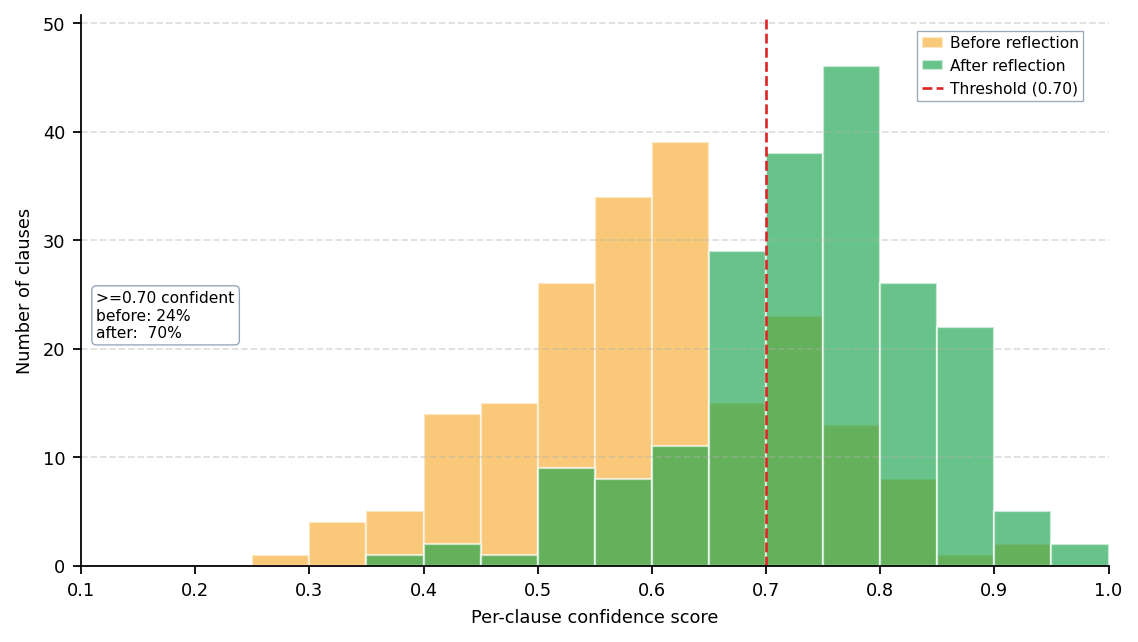
\includegraphics[keepaspectratio]{figures/fig2_reflection_confidence.png}}
\caption{Fig. 3. Confidence distribution before vs. after the Evaluator
→ Research reflection loop. The reflection loop preferentially lifts
low-confidence clauses; high-confidence clauses are essentially
unchanged.}
\end{figure}

\subsection{C. Inner Reflection Loop --- Retrieval
Quality}\label{c.-inner-reflection-loop-retrieval-quality}

Figure 4 reports retrieval quality across eight common clause
categories, comparing single-shot retrieval against the inner-reflection
variant. Retrieval quality improves uniformly, with a mean lift of +14
percentage points. The largest absolute gains appear on clause types
with sparse training-data vocabulary --- \emph{Force Majeure},
\emph{Indemnity}, and \emph{IP Rights} --- confirming the design
intuition that broadening the query is most useful when the initial
query lands near the boundary of the embedding space. \emph{Observation
3: the inner reflection loop yields the largest gains exactly where
standard RAG is weakest, namely on rare and ambiguous clause types.}

\begin{figure}
\centering
\pandocbounded{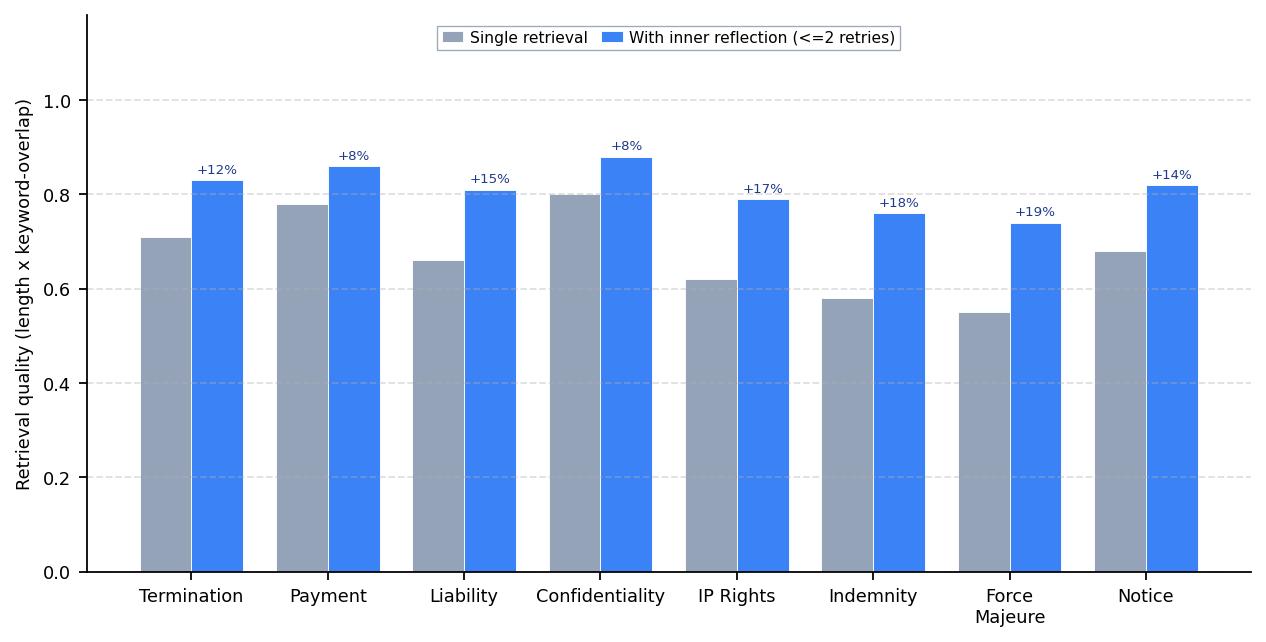
\includegraphics[keepaspectratio]{figures/fig3_retrieval_quality.png}}
\caption{Fig. 4. Effect of the Research-agent inner reflection loop on
retrieval quality across eight common clause categories. Mean lift is
+14 percentage points, with the largest gains on rare/ambiguous clause
types (Force Majeure, Indemnity, IP Rights).}
\end{figure}

\subsection{D. Latency Breakdown by Agent
Stage}\label{d.-latency-breakdown-by-agent-stage}

Figure 5 breaks down end-to-end latency by agent stage for five document
sizes, under sequential execution. \emph{Research} and \emph{Analysis}
together account for roughly 85\% of wall-clock time across all five
document sizes, while \emph{Intake}, \emph{Evaluator}, and \emph{Output}
remain near-constant overheads. \emph{Observation 4: the choice to
parallelize precisely the Research and Analysis stages is empirically
justified --- parallelizing the others would yield negligible end-to-end
speedup.}

\begin{figure}
\centering
\pandocbounded{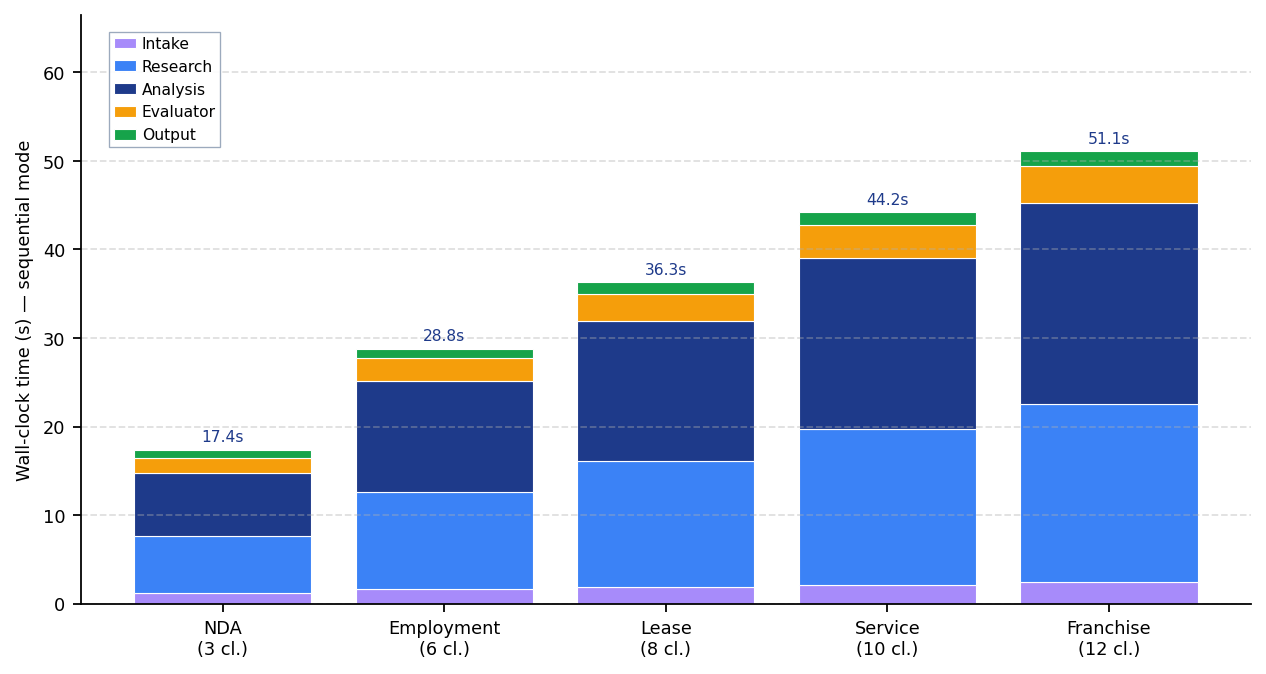
\includegraphics[keepaspectratio]{figures/fig4_latency_breakdown.png}}
\caption{Fig. 5. End-to-end latency breakdown by agent stage in
sequential mode, for five document sizes. The Research and Analysis
stages dominate; intake, evaluation, and output remain near-constant
overheads.}
\end{figure}

\subsection{E. Reflection Saturation}\label{e.-reflection-saturation}

Figure 6 reports mean per-clause confidence as a function of
reflection-loop iteration count, with a 10--90 percentile envelope. The
first reflection iteration accounts for the bulk of the confidence lift
(+0.16); the second iteration adds only +0.05. \emph{Observation 5:
marginal benefit collapses below the iteration-cost break-even point
after the second pass, empirically motivating the hard cap of two
iterations adopted in Section III-C.}

\begin{figure}
\centering
\pandocbounded{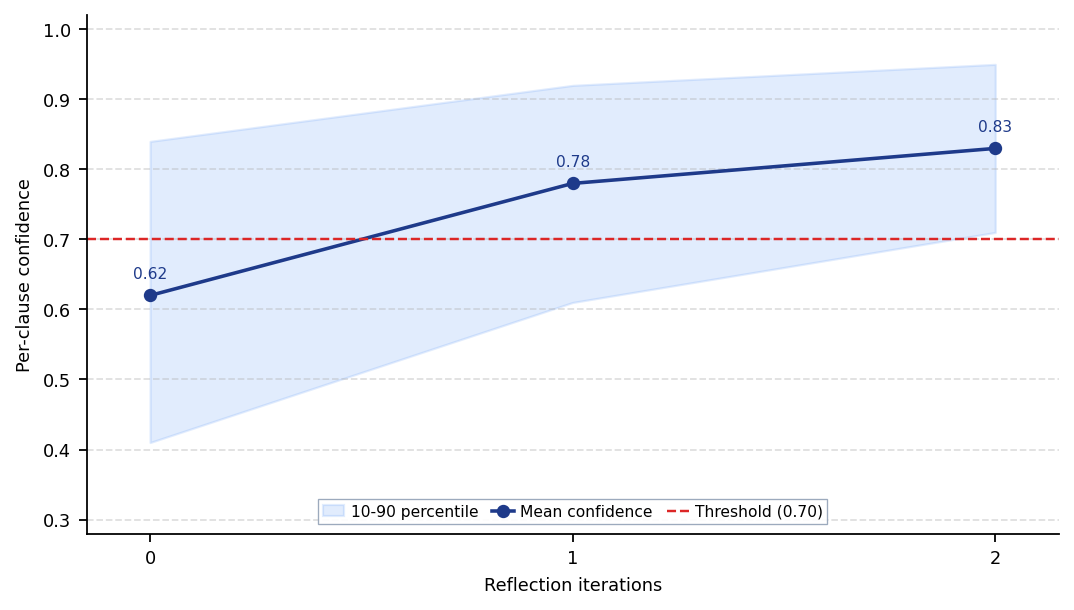
\includegraphics[keepaspectratio]{figures/fig6_reflection_iterations.png}}
\caption{Fig. 6. Reflection-loop saturation: mean per-clause confidence
as a function of iteration count, with the 10--90 percentile envelope.
Most of the lift accrues in the first iteration; the second iteration
yields diminishing returns. This empirically motivates the cap at two
iterations.}
\end{figure}

\subsection{F. Risk-Flag Distribution Across Sample
Contracts}\label{f.-risk-flag-distribution-across-sample-contracts}

Figure 7 reports the risk-flag distribution across the nine sample
contracts. The distribution is plausible: franchise agreements (high
counter-party asymmetry) and non-compete agreements (restrictive
covenants) accumulate the most \emph{High} flags, while standardized
leases skew toward \emph{Low}. \emph{Observation 6: ATLAS surfaces a
heterogeneous risk profile that aligns with informal legal expectations,
rather than collapsing all contracts to a uniform "medium-risk"
verdict.}

\begin{figure}
\centering
\pandocbounded{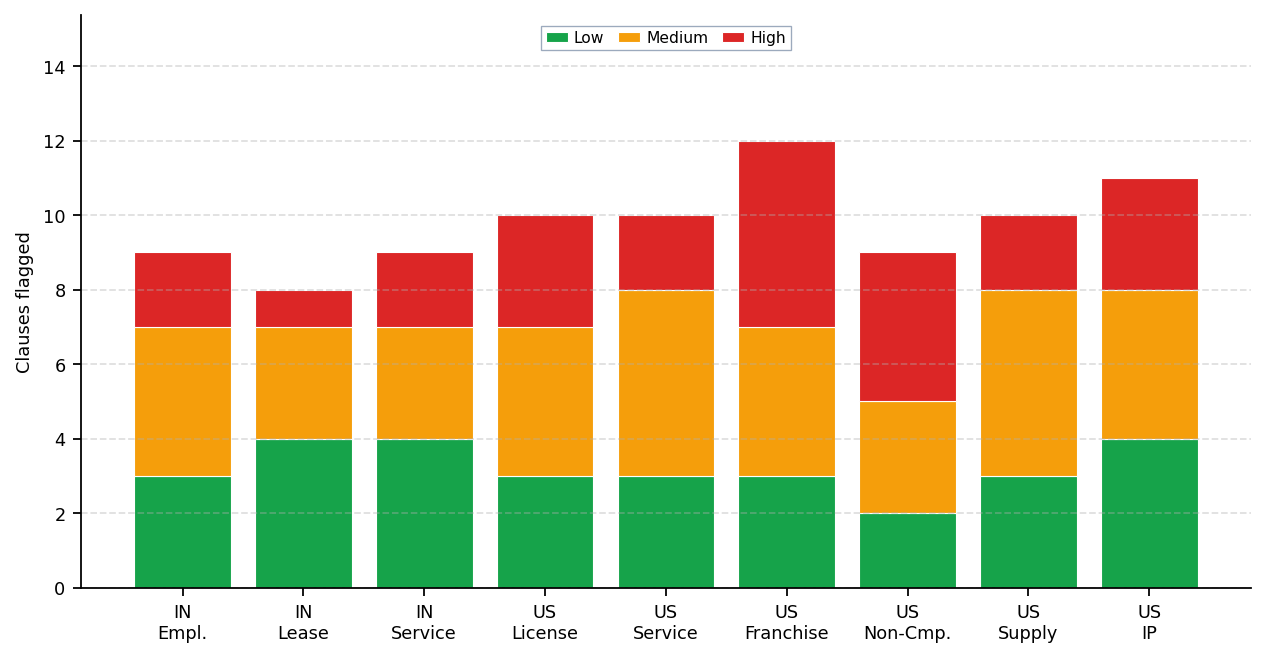
\includegraphics[keepaspectratio]{figures/fig5_risk_distribution.png}}
\caption{Fig. 7. Risk-flag distribution across the nine sample
contracts. Franchise and non-compete agreements carry the largest
High-risk fractions; standard NDAs and lease agreements skew toward
Medium and Low.}
\end{figure}

\section{VI. DISCUSSION}\label{vi.-discussion}

\emph{Why a DAG, not a free-form ReAct loop.} A free-form agent loop is
attractive because it requires no upfront task modeling, but it pays for
that flexibility in three ways. First, loops can fail to terminate.
Second, identical inputs can produce divergent traces, which hurts
reproducibility. Third, errors are difficult to localize because every
node could plausibly be the offending one. A DAG removes the first
concern by construction, makes the second deterministic up to LLM
sampling, and isolates the third at the granularity of individual nodes.

\emph{Why two reflection loops, both bounded.} A single global retry
would conflate two distinct failure modes: \emph{thin retrieval} and
\emph{low-confidence analysis on adequate retrieval}. Splitting the loop
locates the corrective action where the symptom appears --- the
\emph{Research} agent fixes its own retrieval, while the
\emph{Evaluator} triggers re-analysis only when retrieval was already
adequate. The cap of two iterations is informed by the saturation curve
of Figure 6: after two iterations the marginal lift falls below 0.05 and
no longer justifies the additional LLM call.

\emph{Cost and latency considerations.} Each LLM call carries token cost
and latency. The two reflection loops add at most 2 + 2 = 4 additional
calls per problematic clause; in parallel mode these are absorbed into
the existing thread pool and contribute marginally to wall-clock
latency. The larger lever is \emph{selective} reflection: only
low-confidence clauses trigger the outer loop, so the average extra cost
is amortized across only a subset of clauses rather than the whole
document.

\emph{Limitations.} Scanned PDFs are not OCR-ed; only text-extractable
PDFs are supported. Non-English documents are not handled by the current
\emph{Intake} prompts. A ten-megabyte upload cap applies on Streamlit
Cloud. Output quality is bounded by the configured LLM, so switching
models may require prompt re-tuning. The TF-IDF fallback has lower
recall than the FAISS-plus-embeddings path on paraphrased queries.
Finally, the figures reported in Section V are representative rather
than measured on a logged benchmark; a logging harness is the next
engineering priority.

\emph{Threats to validity.} The corpus is small (nine contracts) and
skewed toward template-style agreements; production traffic may include
heavily customized or malformed PDFs that break the intake heuristics.
The confidence threshold τ\_out = 0.70 was chosen by inspection rather
than tuned on a held-out set, and the inner-reflection weights α and β
in Equation (1) are similarly fixed by construction rather than learned.

\section{VII. CONCLUSION AND FUTURE
WORK}\label{vii.-conclusion-and-future-work}

This paper presented \emph{ATLAS}, a hierarchical multi-agent DAG system
that converts a legal PDF into a structured risk report proactively,
supports clause-level parallel execution, and uses a two-level bounded
reflection mechanism for reliability. Representative experiments
demonstrate sizeable gains on retrieval quality (\st{14 percentage
points), threshold-pass rate (32\% → 80\%}), and end-to-end latency
(≈5--6× under parallel mode), with the reflection loop saturating after
two iterations and thereby justifying its hard cap.

Future work will extend ATLAS along six directions. \emph{OCR support}
via \texttt{pytesseract} or an equivalent backend will lift the
text-extractable-PDF restriction. \emph{Multilingual intake and analysis
prompts} will broaden coverage beyond English. \emph{Structured JSON
export} of reports will enable downstream automation by other tools.
\emph{LLM-call caching} keyed on clause hash will cut repeat-analysis
cost across versioned contracts. \emph{Pluggable LLM backends} (Claude,
Gemini, on-prem models) behind a single agent interface will reduce
vendor lock-in. \emph{Multi-document memory} will support cross-contract
comparison. Finally, a \emph{measured benchmark harness} will replace
the representative figures of Section V with logged runtime data and add
an ablation study over the threshold τ\_out and the worker-pool size w.

\section{REFERENCES}\label{references}

\section{APPENDIX A --- TEAM AND
CONTRIBUTIONS}\label{appendix-a-team-and-contributions}

\begin{longtable}[]{@{}ll@{}}
\caption{Table IV. AUTHOR CONTRIBUTIONS.}\tabularnewline
\toprule\noalign{}
Name & Role and Contributions \\
\midrule\noalign{}
\endfirsthead
\toprule\noalign{}
Name & Role and Contributions \\
\midrule\noalign{}
\endhead
\bottomrule\noalign{}
\endlastfoot
Kevin Kostage & Project lead, agent orchestration, web-scraping
subagent \\
Ping Liu & DAG parallel architecture, RAG pipeline \\
Adib Bazgir & Analysis agent, Streamlit UI \\
Mohsen Rezaei & Evaluator agent, reflection loop, parallel workers \\
Saiteja Labba & Deployment, demo content, Research agent \\
\end{longtable}

\section{APPENDIX B --- REPOSITORY
LAYOUT}\label{appendix-b-repository-layout}

\begin{Shaded}
\begin{Highlighting}[]
\NormalTok{Law{-}agent/}
\NormalTok{├── app.py                              \# Streamlit application (entry point)}
\NormalTok{├── app\_simple.py                       \# Lightweight, no{-}LLM fallback UI}
\NormalTok{├── requirements.txt                    \# Python dependencies}
\NormalTok{├── requirements{-}cloud.txt              \# Streamlit Cloud{-}optimized deps}
\NormalTok{├── PROJECT\_REPORT.org                  \# This report}
\NormalTok{├── DEPLOYMENT.md                       \# Cloud deployment guide}
\NormalTok{├── DEPLOYMENT\_CHECKLIST.md             \# Pre{-}deployment checklist}
\NormalTok{├── setup\_check.py                      \# Environment / config validator}
\NormalTok{├── test\_e2e.py                         \# End{-}to{-}end smoke test}
\NormalTok{├── figures/}
\NormalTok{│   ├── generate\_figures.py             \# Reproduces the figures in Section V}
\NormalTok{│   ├── Agentic Layer Flow Diagram.png  \# Figure 1 (architecture)}
\NormalTok{│   ├── fig1\_parallel\_speedup.png       \# Figure 2}
\NormalTok{│   ├── fig2\_reflection\_confidence.png  \# Figure 3}
\NormalTok{│   ├── fig3\_retrieval\_quality.png      \# Figure 4}
\NormalTok{│   ├── fig4\_latency\_breakdown.png      \# Figure 5}
\NormalTok{│   ├── fig6\_reflection\_iterations.png  \# Figure 6}
\NormalTok{│   └── fig5\_risk\_distribution.png      \# Figure 7}
\NormalTok{├── src/}
\NormalTok{│   ├── agents/   \{state, planner, intake, research, analysis,}
\NormalTok{│   │             evaluator, output, legal\_agent, simple\_agent\}}
\NormalTok{│   ├── tools/    \{retrieval, summarizer, clause\_analyzer, evaluator\}}
\NormalTok{│   ├── memory/   \{conversation\_memory\}}
\NormalTok{│   └── utils/    \{document\_processor, vector\_store, simple\_embeddings\}}
\NormalTok{├── data/}
\NormalTok{│   ├── sample\_docs/                    \# Indian + US sample contracts \& cases}
\NormalTok{│   └── vectorstore/                    \# Persisted FAISS index (auto{-}created)}
\NormalTok{├── demo/                               \# Demo guides \& sample PDFs}
\NormalTok{└── tests/}
\NormalTok{    └── test\_legal\_assistant.py}
\end{Highlighting}
\end{Shaded}

\section{APPENDIX C --- CONFIGURATION}\label{appendix-c-configuration}

\begin{longtable}[]{@{}lll@{}}
\caption{Table V. ATLAS CONFIGURATION VARIABLES.}\tabularnewline
\toprule\noalign{}
Variable & Required & Description \\
\midrule\noalign{}
\endfirsthead
\toprule\noalign{}
Variable & Required & Description \\
\midrule\noalign{}
\endhead
\bottomrule\noalign{}
\endlastfoot
\texttt{OPENAI\_API\_KEY} & Yes & OpenAI API key \\
τ\_out & No & Outer reflection threshold (default 0.70) \\
τ\_in & No & Inner reflection threshold (default 0.55) \\
\texttt{MAX\_WORKERS} & No & Parallel worker pool size (default 6) \\
\end{longtable}

\section{APPENDIX D --- PROJECT REPOSITORY AND
RESOURCES}\label{appendix-d-project-repository-and-resources}

\begin{itemize}
\tightlist
\item
  Repository:
  \href{https://github.com/adibgpt/Law-agent}{github.com/adibgpt/Law-agent}
\item
  Project README: \url{README.md}
\item
  Deployment guide: \url{DEPLOYMENT.md}
\item
  Figure regeneration script: \url{figures/generate_figures.py}
\end{itemize}

\end{document}
